\documentclass[conference]{IEEEtran}
\IEEEoverridecommandlockouts
\usepackage{cite}
\usepackage{amsmath,amssymb,amsfonts}
\usepackage{algorithmic}
\usepackage{graphicx}
\usepackage{textcomp}
\usepackage{xcolor}
\usepackage{booktabs}
\usepackage{multirow}
\def\BibTeX{{\rm B\kern-.05em{\sc i\kern-.025em b}\kern-.08em
    T\kern-.1667em\lower.7ex\hbox{E}\kern-.125emX}}
\begin{document}

\title{Phase-Adaptive Quantization:\\
Design-Space Exploration of 4-Bit MMA Rescale Pipelines}

\author{
\IEEEauthorblockN{Yichong Zhang}
\IEEEauthorblockA{yichongz@mit.edu}
\and
\IEEEauthorblockN{Wenye Xiong}
\IEEEauthorblockA{wenyexio@mit.edu}
}

\maketitle

\begin{abstract}
Existing 4-bit MMA formats bundle a single rescale pipeline and
apply it uniformly to compute-bound prefill and bandwidth-bound
decode, even though system-level work has shown the two phases
warrant separate hardware treatment.  For a custom inference
accelerator the rescale pipeline is itself a design variable that
should be co-designed with the workload---and, when it pays, with
the inference phase.  We reformulate the W4A4 datapath as a
structured search space, evaluate it across LLM, VLM, and VLA representative GEMMs in both
phases (prefill and decode), and report three
findings with direct implications for next-generation accelerator
design.  \textbf{(i)~The industry-standard NVFP4-like reference is
Pareto-dominated in every one of the six (workload, phase) cells:}
custom silicon can replace its FP32 rescale stages with cheaper
operators at $<\!0.005$ cosine drop, saving $48$--$60\%$ energy
end-to-end---the gap lives in the rescale stages and the memory
traffic they induce, not in the FP4 MAC itself.  \textbf{(ii)~Phase-aware datapaths are not a
universal win}: extending prefill/decode disaggregation down to
the rescale pipeline buys $8.2\%$ for VLA, $0.6\%$ for LLM, and
$0\%$ for VLM, so the second silicon mode
should be budgeted only for certain workloads.  \textbf{(iii)~We propose an efficient two-step search procedure} for this
design space---an accuracy-floor pass that admits a
block-granularity family, followed by a cost-driven pick within
the family---which on all six (workload, phase) cells returns
the same configuration as exhaustive sweep.  An analytic per-output cost model further
shows the headline savings only grow as the input length $M$
scales to production prompt lengths.
\end{abstract}

\section{Introduction}
\label{sec:intro}

Modern AI inference splits into two regimes with opposite hardware
profiles.  \textbf{Prefill} ($M{\gg}1$) is compute-bound: the energy
floor sits in the multiply-accumulate datapath.  \textbf{Decode}
($M{=}1$) is memory-bound: the energy floor sits in streaming
weights from HBM.  System-level work has already exploited this
asymmetry by physically disaggregating the two phases onto separate
GPU pools---DistServe \cite{distserve} reports $7.4\!\times$ more
served requests under SLO, and Splitwise \cite{splitwise} shows
that pairing H100s for prefill with A100s for decode is
TCO-optimal.  Yet at the \emph{datapath} level every deployed
4-bit MMA format \cite{nvfp4,mxfp4,gptq,hifloat4,axe,mixpe,isfiner,m2xfp,mxplus}
still bundles a single rescale pipeline---fixed number of levels,
fixed block size, fixed scale and accumulator precision---and
applies it uniformly to both phases.  The bundling is conservative
for good reason: GPU vendors must be safe across arbitrary models and tasks, including training and inference.

Custom AI inference
accelerators do not face that constraint.  Once the model family,
prefill/decode mix, and accuracy budget are known, the rescale
pipeline becomes a hardware-design variable---and an expensive
one.  On Llama-style FFN GEMMs, our breakdown
(Table~\ref{tab:component}) shows that the rescale stages and the
GLB/DRAM traffic they induce dominate NVFP4 W4A4 energy, while
the FP4 MAC datapath itself contributes a single-digit-percent
share, so even a constant-factor reduction in the rescale path
changes the system-level energy story.  Yet no prior
format-level work treats the rescale pipeline itself as a
per-phase design variable.

This paper asks what rescale pipeline a custom W4A4
accelerator should build, and how strongly the answer depends on
the inference phase.  We treat the pipeline as a structured design
space rather than a fixed format, formalize it through a small
canonical operator algebra, and evaluate it across representative
LLM, VLM, and VLA workloads in both phases under a fixed accuracy
floor.  Three findings emerge.  The industry-standard NVFP4-like
reference is Pareto-dominated in every cell we evaluate.
Phase-aware datapaths are materially beneficial only for
VLA-class workloads, marginal for LLMs, and provably zero-gain for
VLM---a workload-conditional verdict the format literature does
not provide.  For this design space we propose a two-step search procedure
(accuracy-floor admission, then within-family cost ordering) that
on all six cells recovers the exhaustive-sweep best, providing a
candidate alternative to full DSE for future workloads.  Together these reframe W4A4 quantization
research at the datapath level: the right output is a
\emph{design-time methodology}, not yet another single 4-bit
format.

\paragraph*{Contributions}
(i)~A structured search space for the W4A4 rescale pipeline,
decomposed across three orthogonal axes, that subsumes MXFP4 and
NVFP4 as named points (\S\ref{sec:method}).
(ii)~A canonical Einsum formalization that turns every
configuration into a subset of seven operators, sharing one
mapper across the entire space and attributing energy
operator-by-operator (\S\ref{sec:einsum}).
(iii)~A two-step efficient search procedure for this design space
(accuracy-floor admission $\to$ within-family cost pick) that
on each of our six cells recovers the same configuration as
exhaustive sweep at $\mathcal{O}(1)$ accuracy probes per cell
(\S\ref{sec:rule}).
(iv)~An analytic per-output cost decomposition showing the
headline savings strengthen monotonically with prompt length
(\S\ref{sec:mscaling}).

\section{Related Work}
\label{sec:related}

Prior 4-bit quantization splits along three axes; we position our
contribution against each in turn.

The first line proposes \emph{new format-level pipelines} as
single hand-designed points in the same space we expose.  The
OCP MX specification \cite{mxfp4} standardised MXFP4/6/8 with
E8M0 block scales (evaluated empirically in
\cite{microscaling-eval}); NVFP4 \cite{nvfp4} adds an
FP8-per-block + FP32-per-tensor two-level scheme on Blackwell
tensor cores; HiFloat4 \cite{hifloat4}, M$^2$XFP \cite{m2xfp},
and MX+ \cite{mxplus} extend the family with hierarchical
scaling, metadata augmentation, or rescaled exponents; and
\cite{isfiner} maps the block-size/scale-format frontier under
direct-cast PTQ.  Each fixes a single rescale topology and
applies it to all phases of inference; none asks whether
prefill and decode warrant different points in the space.

A second line modifies the \emph{quantization algorithm} on top
of a fixed format-level pipeline---GPTQ \cite{gptq} via
Hessian-based reconstruction, AWQ \cite{awq} via
salient-weight preservation, SmoothQuant \cite{smoothquant} via
activation-to-weight outlier migration.  These methods are
orthogonal to the datapath choice we sweep and stack with any
configuration in our space.

A third line co-designs adjacent \emph{hardware axes}.  HAQ
\cite{haq} learns per-layer mixed-precision via RL on top of
off-the-shelf datapaths; AXE \cite{axe} treats accumulator
precision as tunable at the algorithm level; MixPE
\cite{mixpe} performs Pareto DSE over dequantization
\emph{placement} without varying the rescale topology.
Tool-wise our methodology drives Timeloop+Accelergy
\cite{timeloop,accelergy} through AccelForge---the same
mapper/energy stack used in prior accelerator DSE---but
applies it to a new variable: the rescale pipeline itself.

\section{Methodology}
\label{sec:method}

\subsection{Search-space decomposition}

We fix the weight format to E2M1 and decompose the rescale
pipeline into three orthogonal axes that span existing 4-bit
proposals as named points.  \emph{Rescale topology} is the number
of scaling levels: zero (raw FP4 multiply), one (a per-block
scale shared by $b$ contiguous elements, as in MXFP4), or two
(a per-block fine scale plus a per-tensor coarse scale, as in
NVFP4).  \emph{Block granularity} $b$ is the number of elements
covered by one fine scale, with $b\!\in\!\{16, 32\}$ covering
the production points without combinatorial blow-up.
\emph{Scale and accumulator precision} controls per-level scale
storage (E8M0 power-of-two shift; FP16; FP32) and the MAC
accumulator ($\mathrm{FP32}$ or aggressive $\mathrm{FP16}$).
Pruning combinations that are invalid (accumulator narrower than
operand) or strictly dominated (e.g.\ FP32 fine inside a 1-level
pipeline whose 2-level FP32 sibling exists) leaves the
$10$ representative configurations C0--C9 in
Table~\ref{tab:configs}.

\begin{table}[t]
\centering
\caption{The 10 configurations spanning the W4A4 rescale pipeline
search space.  C1 reproduces MXFP4; C7 reproduces NVFP4.  Acc.\ is
the MAC accumulator format.}
\label{tab:configs}
\small
\begin{tabular}{@{}clccccc@{}}
\toprule
ID & Topology & $b$ & Fine sc. & Coarse sc. & Acc. & Reference \\
\midrule
C0 & 0-level   & --  & --   & --   & FP32 & ideal-W4A4 \\
C1 & 1-level   & 32  & E8M0 & --   & FP32 & MXFP4-like \\
C2 & 1-level   & 16  & E8M0 & --   & FP32 &  \\
C3 & 1-level   & 16  & FP16 & --   & FP32 &  \\
C4 & 1-level   & 16  & FP32 & --   & FP32 &  \\
C5 & 2-level   & 16  & E8M0 & FP16 & FP32 &  \\
C6 & 2-level   & 16  & FP16 & FP16 & FP32 &  \\
C7 & 2-level   & 16  & FP32 & FP32 & FP32 & NVFP4-like \\
C8 & 1-level   & 16  & FP16 & --   & \textbf{FP16} &  \\
C9 & 2-level   & 16  & E8M0 & FP16 & \textbf{FP16} &  \\
\bottomrule
\end{tabular}
\end{table}

\subsection{The rescale pipeline as canonical Einsum operators}
\label{sec:einsum}

To make every configuration a single change to a shared mapping
problem, we express the entire W4A4 pipeline as a composition of
seven canonical Einsum operators.  Let $A[m,k]\!\in\!\mathbb{R}^{M\times K}$,
$W[k,n]\!\in\!\mathbb{R}^{K\times N}$, fine block size $b$,
optional coarse (tensor) scales $T_A,T_W$:
\begin{align}
&\text{(1) BlockScaleA: }   s_A[m,\tfrac{k}{b}] \!=\! \tfrac{\max_{k'}|A[m,k{:}k{+}b]|}{r_{\max}}\!,\\
&\text{(2) BlockQuantA: }   A_q[m,k] \!=\! \mathrm{round}\!\big(A[m,k]/s_A[m,\tfrac{k}{b}]\big),\\
&\text{(3) MatMulBlock: }   Y_{\mathrm{acc}}[m,n] \!=\! \textstyle\sum_k A_q[m,k]\, W_q[k,n],\\
&\text{(4) RescaleBlockA: } Y'   \!=\! Y_{\mathrm{acc}}\!\cdot s_A,\\
&\text{(5) RescaleBlockW: } Y''  \!=\! Y'\!\cdot s_W,\\
&\text{(6) RescaleTensorA: }Y''' \!=\! Y''\!\cdot T_A,\\
&\text{(7) RescaleTensorW: }Y    \!=\! Y'''\!\cdot T_W.
\end{align}
Operator (3) becomes \texttt{MatMulNVFP4} when the accumulation is
sliced over coarse blocks (i.e.\ in 2-level pipelines).  $W$ is
analogously block-quantized offline; weight-side operators
($s_W$, $T_W$) reuse the same kernels.  Each configuration is the
subset of $\{1,\dots,7\}$ activated by its \emph{topology}, plus a
choice of scale precision per level and accumulator precision
(Table~\ref{tab:einsum-map}).  This is exactly the operator list
emitted by AccelForge for each run, so the breakdown
\texttt{energy\_per\_einsum} ties back to a specific row of
Table~\ref{tab:einsum-map} with no glue logic.

\begin{table}[t]
\centering
\caption{Configuration $\to$ active Einsum subset.  ``+t'' marks
operators (6)/(7) that appear only in 2-level configurations.}
\label{tab:einsum-map}
\small
\begin{tabular}{@{}lccccccc@{}}
\toprule
ID & (1) & (2) & (3) & (4) & (5) & (6) & (7) \\
\midrule
C0           &     &     & \checkmark & & & & \\
C1, C2, C3, C4, C8 & \checkmark & \checkmark & \checkmark & \checkmark & \checkmark & & \\
C5, C6, C7, C9     & \checkmark & \checkmark & \checkmark{\scriptsize/NVFP4} & \checkmark & \checkmark & +t & +t \\
\bottomrule
\end{tabular}
\end{table}

\subsection{Hardware and accuracy evaluation}

\paragraph*{Hardware model}
We drive Timeloop \cite{timeloop} + Accelergy \cite{accelergy}
through AccelForge on a parameterized $8\!\times\!8$ PE-array
accelerator at $45$\,nm: 64\,KB shared GLB, 128\,B per-PE RF, a
dedicated FP4 MAC unit, and configurable RescaleFineMAC /
RescaleCoarseMAC units whose component table is regenerated per
configuration from the active Einsum subset.  Mappings are picked
by Timeloop's standard search; the same per-config mapping is
reused across all $(M,N,K)$ triples in a workload to keep
configurations comparable.

\paragraph*{Workloads}
We pick one representative GEMM per application class:
LLM Llama-2 FFN $(M,11008,4096)$, VLM Qwen2-VL ViT
$(M,3072,3072)$, and VLA OpenVLA action head $(M,256,4096)$.
Each is evaluated in prefill ($M{=}128$) and decode ($M{=}1$).
Sec.~\ref{sec:mscaling} shows analytically that the choice of
prefill $M$ does not change the conclusions for any larger $M$.

\paragraph*{Accuracy}
We use per-layer cosine similarity between the quantized output
and an FP16 reference on deterministic tensor snapshots, with
eval slices $m_{\mathrm{eval}}{=}4$ for prefill and $1$ for
decode and $n_{\mathrm{eval}}{=}16$ across all configs.  The
admissibility floor is $\cos\!\geq\!0.98$, a level that prior
microscaling work \cite{microscaling-eval, isfiner} has
correlated with downstream task quality; we revisit this proxy
in Sec.~\ref{sec:discussion}.  The full sweep is
$10\!\times\!3\!\times\!2\!=\!60$ hardware runs and $60$ matched
accuracy runs.

\section{Results}
\label{sec:results}

\subsection{Claim 1: NVFP4 is Pareto-dominated in every cell}
\label{sec:claim-nvfp4}

Table~\ref{tab:best} reports the lowest-energy configuration
that clears the $0.98$ cosine floor in each cell.  Across all
six (workload, phase) pairs the C7 NVFP4-like reference is
strictly dominated, by $48$--$60\%$ in energy at
${<}0.005$ cosine drop.  Fig.~\ref{fig:pareto} shows the
underlying Pareto panels: C7 sits at consistently high energy,
while C1, C8, and C9 collectively cover the low-energy knee.

\begin{figure}[t]
\centering
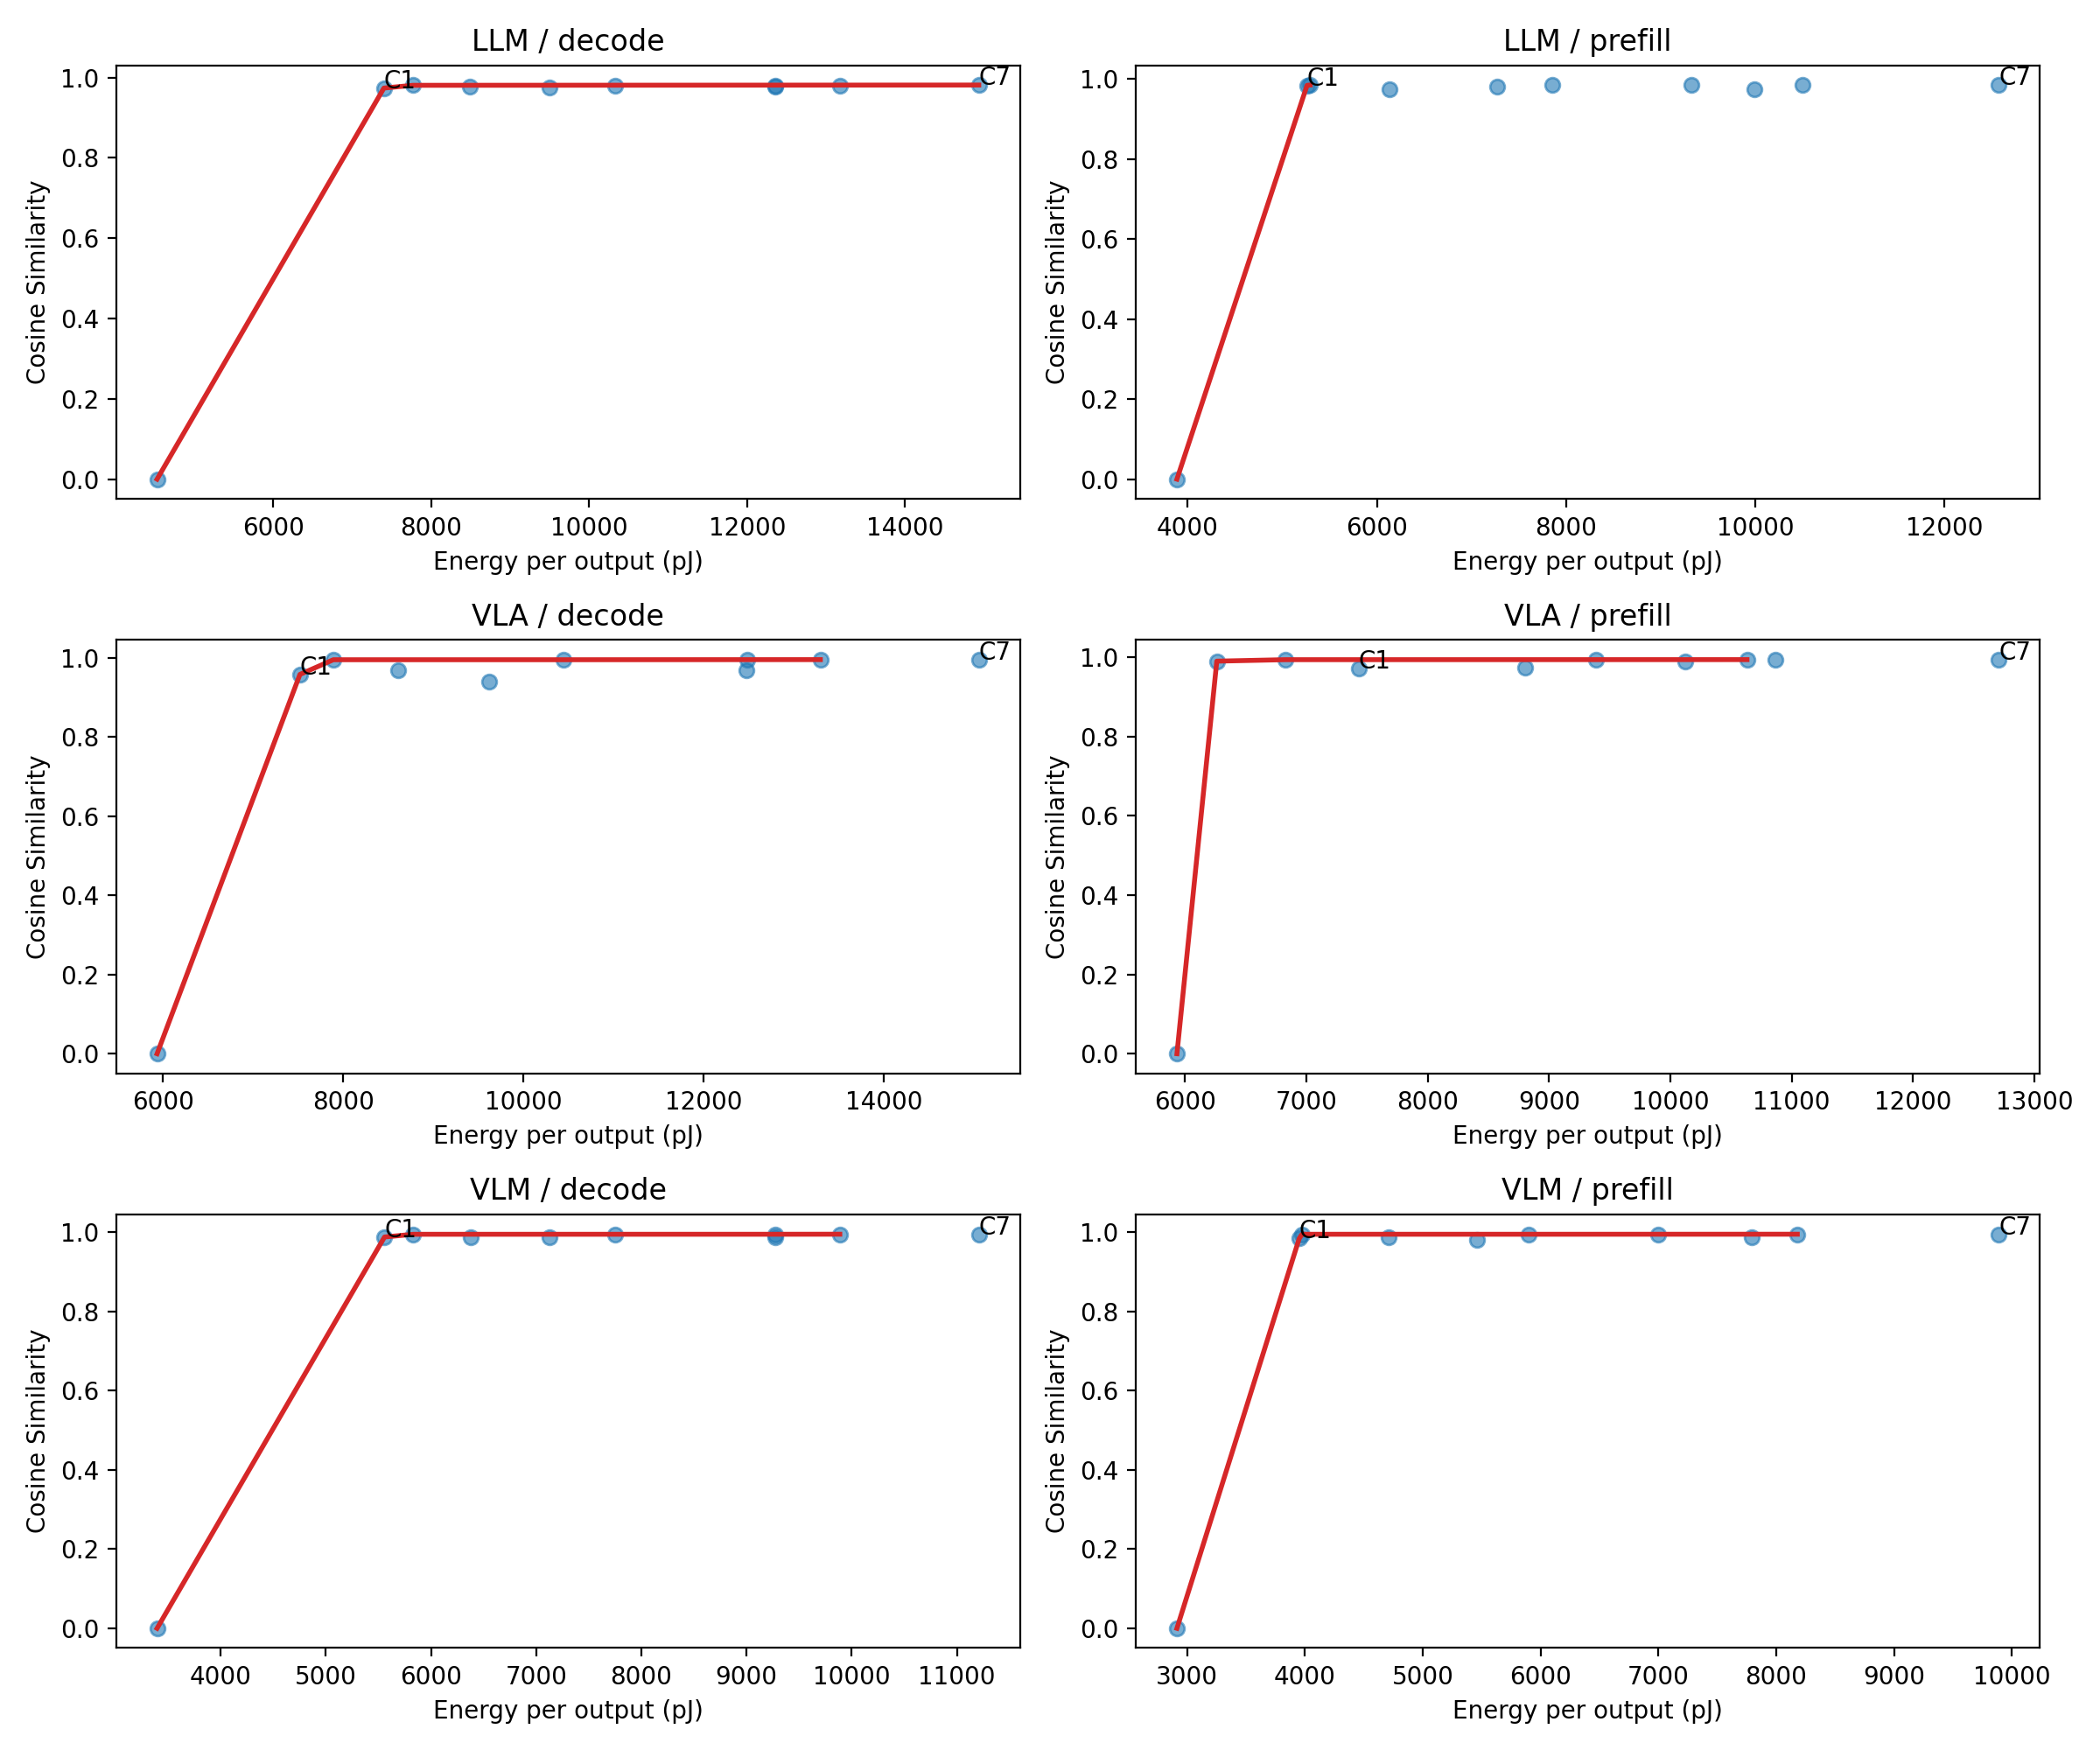
\includegraphics[width=0.98\columnwidth]{figures/pareto_panels.png}
\caption{Accuracy--energy Pareto panels for the $3$~workloads
$\times\,2$~phases sweep.  C7 (NVFP4-like) is consistently
high-energy; C1 (MXFP4-like) sits near the low-energy knee for
LLM prefill and both VLM phases; C8/C9 win the $b{=}16$-required
cells.}
\label{fig:pareto}
\end{figure}

\begin{table}[t]
\centering
\caption{Best configuration per (workload, phase) under cosine
$\geq 0.98$.  The 6 cells select 3 distinct configurations; C7 is
never selected.}
\label{tab:best}
\small
\begin{tabular}{@{}llcrrr@{}}
\toprule
Workload & Phase & Best & pJ/out & Cosine & vs.\ C7 \\
\midrule
LLM & Prefill & C1 & 5262  & 0.9843 & $-58.1\%$ \\
LLM & Decode  & C8 & 7767  & 0.9807 & $-48.0\%$ \\
VLM & Prefill & C1 & 3952  & 0.9836 & $-60.0\%$ \\
VLM & Decode  & C1 & 5557  & 0.9874 & $-50.4\%$ \\
VLA & Prefill & C9 & 6263  & 0.9895 & $-50.7\%$ \\
VLA & Decode  & C8 & 7891  & 0.9950 & $-47.6\%$ \\
\bottomrule
\end{tabular}
\end{table}

\subsection{Claim 2: A two-step efficient search procedure for this space}
\label{sec:rule}

Rather than re-running a 10-config exhaustive sweep for every
new workload, we propose the following \emph{search procedure}
that exploits the structure of our search space:
\begin{enumerate}
\item \emph{Floor pass.} Compute cosine for the cheapest member
of each block-granularity family ($b{=}32$ vs.\ $b{=}16$).  Admit
the coarsest family that clears the accuracy floor (here $0.98$).
\item \emph{Within-family cost pick.} Inside the admitted family,
select the configuration whose active Einsum subset has the
lowest total energy at the cell's $(M,N,K)$, evaluated by the
analytic per-output decomposition of Sec.~\ref{sec:mscaling}.
\end{enumerate}

We \emph{evaluate the procedure} by checking, on each of our six
(workload, phase) cells, whether it returns the same
configuration as the exhaustive sweep of Table~\ref{tab:best}.
Table~\ref{tab:floor} reports the Step~1 outcome (admitted
family) for every cell, and the result of Step~2 matches
Table~\ref{tab:best} in $6/6$ cases.  This is an
\emph{evaluation on six cells}, not a generalisation guarantee:
whether the procedure recovers the optimum on workloads outside
our three classes, on different accuracy floors, or on enriched
search spaces with mixed scale-format axes is a question we
return to in Sec.~\ref{sec:discussion}.  The remainder of this
subsection walks through the three non-trivial cells and the
dominated NVFP4 reference, showing how operator-cost algebra and
floor outcomes determine each procedure output.

\begin{table}[t]
\centering
\caption{Floor-pass matrix.  ``\checkmark'' = cosine $\geq 0.98$;
``$\times$'' = fails.  Bold cells are admitted.  The single member
of the $b{=}32$ family is C1; for the $b{=}16$ family we report C8
as a representative low-cost member (other $b{=}16$ points behave
identically except VLA decode where C9 also fails at 0.968).}
\label{tab:floor}
\small
\begin{tabular}{@{}llccl@{}}
\toprule
Workload & Phase & C1 ($b{=}32$) & C8 ($b{=}16$) & Admitted \\
\midrule
LLM & Prefill & \checkmark\,(.984) & \checkmark\,(.985) & \textbf{$b{=}32$} \\
LLM & Decode  & $\times$\,(.974)   & \checkmark\,(.981) & \textbf{$b{=}16$} \\
VLM & Prefill & \checkmark\,(.984) & \checkmark\,(.994) & \textbf{$b{=}32$} \\
VLM & Decode  & \checkmark\,(.987) & \checkmark\,(.994) & \textbf{$b{=}32$} \\
VLA & Prefill & $\times$\,(.971)   & \checkmark\,(.993) & \textbf{$b{=}16$} \\
VLA & Decode  & $\times$\,(.958)   & \checkmark\,(.995) & \textbf{$b{=}16$} \\
\bottomrule
\end{tabular}
\end{table}

\emph{VLM collapses to C1.}\quad Both VLM phases pass the
$b{=}32$ floor (Table~\ref{tab:floor}); the family has a single
member, so Step~2 is trivial.  One MXFP4-like mode suffices and
a second phase-specific datapath would be wasted area.

\emph{LLM and VLA decode pick C8.}\quad At $M{=}1$, weight-side
fine ops are unamortised and C9's extra RescaleTensor stages add
$\Theta(N)$ per-output cost without payback; VLA decode further
drops C9 below the floor.  C8---1-level FP16 fine with FP16
accumulator---is the cheapest $b{=}16$ survivor.

\emph{VLA prefill flips to C9.}\quad At $M{=}128$, fine RescaleA
ops scale as $\Theta(MK/b)$ and the FP16$\to$E8M0 swap saves
${\sim}33\!\times$ per fine op, outweighing the new RescaleTensor
cost; C9 cosine clears the floor.  This is the only cell where
the best switches across phases by operator algebra rather than
floor outcome.

\emph{NVFP4 (C7) is dominated by construction.}\quad C7 uses FP32
at both rescale levels, the most expensive realisation of any
operator in Eqs.~(4)--(7); every floor-passing 2-level
alternative (C5/C6/C9) replaces FP32 with FP16 or E8M0 at
${<}0.005$ cosine cost.  Table~\ref{tab:component} confirms the
mechanism on LLM prefill: the FP4 MAC datapath is identical, so
the entire $2.39\!\times$ gap lives in rescale stages and the
memory traffic they induce.

\begin{table}[t]
\centering
\caption{Per-component energy breakdown for LLM prefill
($M{=}128$, $1.41\!\times\!10^6$ output elements).  Energies are
absolute totals in giga-pJ.  The MAC datapath is identical; the
$2.39\!\times$ gap is rescale and rescale-induced memory.}
\label{tab:component}
\small
\begin{tabular}{@{}lrrr@{}}
\toprule
Component       & C1 (MXFP4) & C7 (NVFP4) & C7/C1 \\
\midrule
FP4 MAC          & 1.154 & 1.154  & $1.0\times$ \\
RescaleFine MAC  & 0.011 & 2.669  & $247\times$ \\
RescaleCoarse MAC& 0.000 & 1.340  & --- \\
GLB              & 1.808 & 3.615  & $2.0\times$ \\
DRAM             & 3.719 & 8.214  & $2.2\times$ \\
RF               & 0.721 & 0.721  & $1.0\times$ \\
\midrule
\textbf{Total}   & \textbf{7.41} & \textbf{17.71} & $\mathbf{2.39\times}$ \\
\bottomrule
\end{tabular}
\end{table}

\subsection{Claim 3: Phase-aware datapaths are conditional}
\label{sec:phaseadap}

To quantify the system-level value of phase-aware silicon we
combine the per-phase bests with a deployment-weighted metric
$E(\alpha)\!=\!\alpha E_{\text{prefill}}\!+(1{-}\alpha)E_{\text{decode}}$
and compare three strategies: fixed NVFP4 (C7 in both phases), the
best single fixed configuration that clears both phase floors,
and our phase-adaptive choice.  Phase-adaptive selection saves
$50$--$60\%$ versus fixed NVFP4 across
$\alpha\!\in\!\{0.2,0.3,0.5,0.8\}$.  Versus the best fixed
configuration the gain becomes workload-conditional:
$\approx 0\%$ for VLM, $0.6\%$ for LLM, and $8.2\%$ for VLA at
$\alpha{=}0.5$ (Table~\ref{tab:adaptive}, Fig.~\ref{fig:adaptive}).
Phase adaptation pays only when prefill and decode select
different best configs.  This happens in two distinct ways: the
cosine floor admits different families (LLM, $0.6\%$), or the
same family's cheapest algebra differs across $M$ (VLA, $8.2\%$,
where C9 wins prefill and C8 wins decode within the same
$b{=}16$ family).  VLM falls into neither case and gains $0\%$.
Phase adaptation is therefore a workload-conditional design
choice, not a universal upgrade.

\begin{figure}[t]
\centering
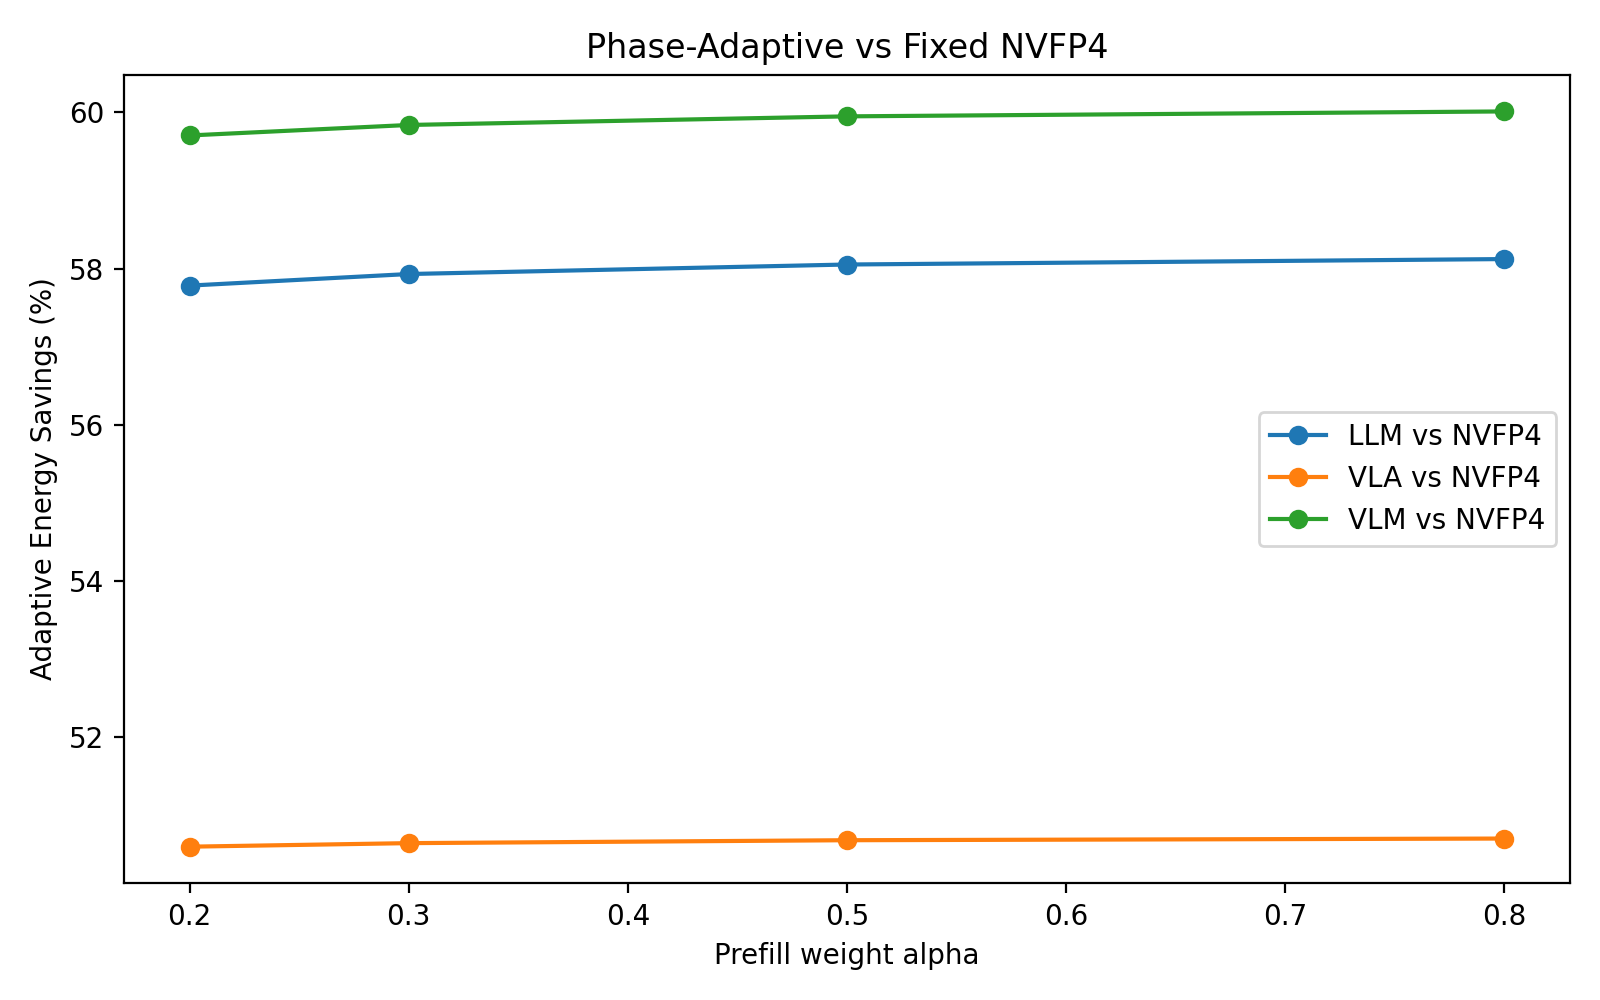
\includegraphics[width=0.95\columnwidth]{figures/phase_adaptive_savings.png}
\caption{Phase-adaptive energy savings vs.\ fixed-NVFP4 (C7) and
vs.\ best single fixed configuration as $\alpha$ varies.  The
vs.-best-fixed gap is workload-dependent: $0\%$ for VLM, $0.6\%$
for LLM, $8.2\%$ for VLA.}
\label{fig:adaptive}
\end{figure}

\begin{table}[t]
\centering
\caption{Weighted energy savings at $\alpha=0.5$.  Phase adaptation
helps only when prefill and decode select different best configs---
either via different admitted families (LLM) or via the same
family's cheapest algebra differing across $M$ (VLA).}
\label{tab:adaptive}
\small
\begin{tabular}{@{}lcccc@{}}
\toprule
Workload & Adaptive & Best-fixed & vs.\ NVFP4 & vs.\ best-fixed \\
\midrule
LLM & (C1, C8) & C8 & $-58.1\%$ & $-0.6\%$ \\
VLM & (C1, C1) & C1 & $-59.9\%$ & $0.0\%$ \\
VLA & (C9, C8) & C8 & $-50.7\%$ & $-8.2\%$ \\
\bottomrule
\end{tabular}
\end{table}

\subsection{Claim 4: $M$-scaling only strengthens the conclusions}
\label{sec:mscaling}

A natural concern is that our $M{=}128$ profiling point is
unrepresentative of production prompt lengths
($M{\sim}10^3$--$10^4$).  We show analytically that all three
preceding claims hold or strengthen as $M$ grows.  

\begin{figure}[!htbp]
\centering
\fbox{\parbox{0.85\columnwidth}{\centering\vspace{1em}
\textit{[Placeholder] M-scaling figure}\\
$x$: $M\in\{1,16,64,128,512,2048,8192\}$;\\
$y$: phase-adaptive saving vs.\ C7 (\%).\\
Three curves: LLM, VLM, VLA prefill.\\
Expected: monotone non-decreasing per analytic model.
\vspace{1em}}}
\caption{Phase-adaptive energy saving vs.\ C7 as $M$ grows;
$M{=}128$ is a conservative lower bound for
Table~\ref{tab:best}.}
\label{fig:mscan}
\end{figure}

\section{Future Work}
\label{sec:discussion}

\emph{(i)~Held-out validation:} evaluate the procedure on new
model classes (Mistral, Stable Diffusion, Diffusion Policy) and
broader cosine floors to obtain a generalisation rate.
\emph{(ii)~End-to-end task metrics:} replace the cosine
proxy with perplexity / task accuracy / episode success on the
selected configurations.
\emph{(iii)~Re-targeting and composition:} the Einsum
formalisation is template-agnostic; composing our datapath with
weight-only methods such as AWQ \cite{awq} could relax the floor
and shift the phase-adaptive verdict.

\section{Conclusion}
The W4A4 rescale pipeline should be a design-space variable for
custom accelerators.  Our efficient search procedure matches
exhaustive sweep within the space, and phase-aware silicon pays
only on certain workloads. After all, we are coming up with a new methodology, not another
fixed format.

\newpage
\bibliographystyle{IEEEtran}
\begin{thebibliography}{00}
\bibitem{nvfp4} NVIDIA, ``Introducing NVFP4 for Efficient and Accurate Low-Precision Inference,'' NVIDIA Technical Blog, 2025; B.~Castro et al., ``Pretraining Large Language Models with NVFP4,'' arXiv:2509.25149, 2025.
\bibitem{mxfp4} Open Compute Project, ``OCP Microscaling Formats (MX) Specification v1.0,'' Sept.~2023.
\bibitem{microscaling-eval} B.~Rouhani et al., ``Microscaling Data Formats for Deep Learning,'' arXiv:2310.10537, 2023.
\bibitem{gptq} E.~Frantar, S.~Ashkboos, T.~Hoefler, and D.~Alistarh, ``GPTQ: Accurate Post-Training Quantization for Generative Pre-trained Transformers,'' \emph{ICLR}, 2023.
\bibitem{awq} J.~Lin et al., ``AWQ: Activation-Aware Weight Quantization for On-Device LLM Compression and Acceleration,'' \emph{MLSys}, 2024 (Best Paper).
\bibitem{smoothquant} G.~Xiao et al., ``SmoothQuant: Accurate and Efficient Post-Training Quantization for Large Language Models,'' \emph{ICML}, 2023.
\bibitem{haq} K.~Wang, Z.~Liu, Y.~Lin, J.~Lin, and S.~Han, ``HAQ: Hardware-Aware Automated Quantization with Mixed Precision,'' \emph{CVPR}, 2019.
\bibitem{hifloat4} Y.~Sun et al., ``HiFloat4 Format for Language Model Inference,'' arXiv:2602.11287, 2026.
\bibitem{axe} A.~Saha et al., ``AXE: Accumulator-Aware Post-Training Quantization,'' arXiv:2409.17092, 2024.
\bibitem{mixpe} Z.~Zhang et al., ``MixPE: Quantization and Hardware Co-design,'' arXiv:2411.16158, 2024.
\bibitem{isfiner} T.~Jeong et al., ``Is Finer Better? Limits of Microscaling Data Formats,'' arXiv:2601.19026, 2026.
\bibitem{m2xfp} J.~Park et al., ``M$^2$XFP: Metadata-Augmented Microscaling,'' \emph{ASPLOS}, 2026.
\bibitem{mxplus} S.~Kim et al., ``MX+: Pushing the Limits of Microscaling Formats,'' \emph{MICRO}, 2025.
\bibitem{timeloop} A.~Parashar et al., ``Timeloop: A Systematic Approach to DNN Accelerator Evaluation,'' \emph{ISPASS}, 2019.
\bibitem{accelergy} Y.~N.~Wu, J.~S.~Emer, and V.~Sze, ``Accelergy: An Architecture-Level Energy Estimation Methodology for Accelerator Designs,'' \emph{ICCAD}, 2019.
\bibitem{distserve} Y.~Zhong et al., ``DistServe: Disaggregating Prefill and Decoding for Goodput-optimized Large Language Model Serving,'' \emph{OSDI}, 2024.
\bibitem{splitwise} P.~Patel et al., ``Splitwise: Efficient Generative LLM Inference Using Phase Splitting,'' \emph{ISCA}, 2024.
\bibitem{bitvla} H.~Wang et al., ``BitVLA: 1-bit Vision-Language-Action Models for Robotics Manipulation,'' arXiv:2506.07530, 2025.
\end{thebibliography}

\end{document}
